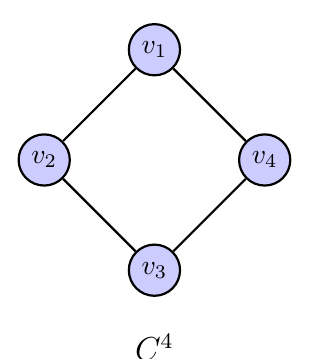
\begin{tikzpicture}[
  baseline=0pt,
  scale=0.7,
  vnode/.style={circle, draw=black, fill=blue!20, thick, inner sep=0pt, minimum size=6.5mm},
  edge/.style={thick, draw=black}
]
  \useasboundingbox (-2.3,-3.1) rectangle (2.3,2.4);

  % Vértices en radio 2.0 cm (v1 a 90°, v3 a 270°)
  \node[vnode] (v1) at (90:2.0) {$v_1$};
  \node[vnode] (v2) at (180:2.0) {$v_2$};
  \node[vnode] (v3) at (270:2.0) {$v_3$};
  \node[vnode] (v4) at (0:2.0) {$v_4$};

  % Aristas del ciclo C^4
  \draw[edge] (v1) -- (v2) -- (v3) -- (v4) -- (v1);

  % Etiqueta inferior en tamaño normal
  \node at (0,-3.4) {\large{$C^4$}};
\end{tikzpicture}
